\chapter{Gesamtsystem}

\section{Komponentendiagramm}
Abbildung \ref{pic:component_diag} zeigt die fachliche Aufteilung der Softwarekomponenten. Es lassen sich drei Schichten ableiten. An oberster Stelle steht die Webapp mit den Templates 
aller Seiten und Unterseiten. Diese Templates greifen auf die Controller der Komponenten darunter zu. Jede Komponente, also wettbewerbe, mannschaften, spieler und login beinhalten ihre 
eigenen Controller in einem Controller Paket. Ausser dem Controller Paket befindet sich noch ein Paket für die Modelklassen, ein Paket für die Producer, welche Objekte erzeugen die injected werden 
können und ein Servicepaket zur Kommunikation mit der Datenbank jeder Komponente. Die unterste Schicht, die persistance Komponente schreibt und liest Daten aus einer H2 Datenbank mit Hilfe 
des JPA-Frameworks. 




%In der Abbildung \ref{pic:component_diag} ist die Übersicht der Systembausteine dargesstellt. 
%Das System selbst ist in drei Schichten aufgeteilt. Eine Schicht, für die Benutzeroberfläche, die Steuereinheiten und Oberflächenelemente enthält.
%Eine Schicht für das Datenmodell und eine Schicht für die Daten-Persistenz.\\
%\\
%Innerhalb der Schichten, gibt es zwei rot markierte Komponenten. Die \enquote{ObjectTemplate-Komponente} und  die \enquote{DataModel-Komponente}. 
%Diese stellen die Elemente dar, die an den spezifischen Anwendungsfall angepasst werden müssen. 
%Die \enquote{Datamodel}-Komponente entspricht dem tatsächlichen Datenmodel der Anwendung. 
%Alle Elemente, die vom Framework dargestellt werden sollen, müssen das Viewable-Interface aus der \enquote{AbstractModel}-Komponente implementieren.
%Zusätlich müssen für alle Elemente des Datenmodells eigenene Frontend-Template erstellt werden, welche ein bestimmtes Namensschema befolgen - Die \enquote{Object-Templates}. 
%Ein einheitliches Namensschema löst das Problem mit unterschiedlichen Darstellungsmöglichkeiten. Innerhalb der Templates ist es möglich 
%Validierungskriterien für die Element-Attribute zu formulieren, wodurch die Konsistenz des Datenbestandes gesichert werden soll.\\
%\\
%Die Steurungselemente des User-Interfaces, sowie die Templates, arbeiten mit
%den Elementen der \enquote{AbstractModel}-Komponente. Dies ermöglicht einen Austausch des Datenmodels der Anwendung. 
%Damit der Datenbestand persistiert werden kann, setzt das Framework voraus, dass jedes Viewable-Element eine Entity des JPA-Frameworks ist. Das \enquote{Loader}-Element der \enquote{Controller}-Komponente 
%greift direkt auf das JPA zu, um die Daten in der Datenbank zu verwalten. Es arbeitet jedoch immer nur mit den \enquote{Viewable}-Elementen. 

%Für die Formatierung der Abbildung -> newpage -> sonst springt es wohin es will.
%\newpage

\begin{figure}[H]
	\caption{Komponenten Diagramm}
	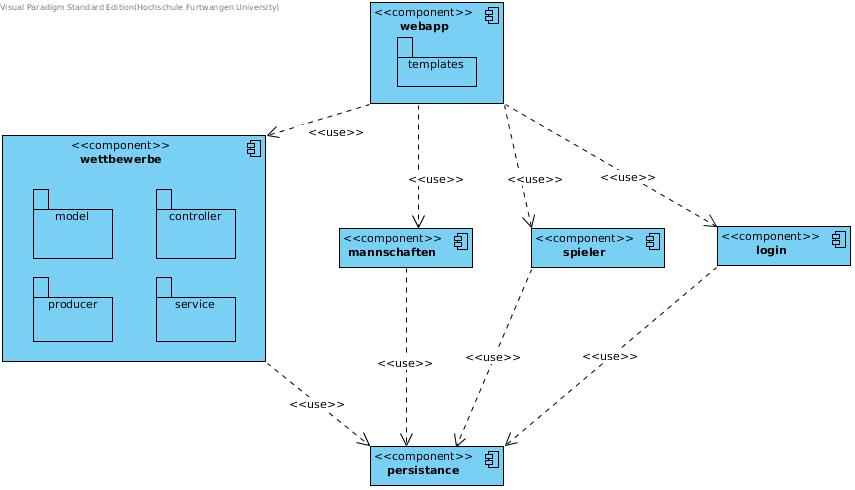
\includegraphics[width=0.9\textwidth]{content/pictures/komponentendiagramm}
	\label{pic:component_diag}
\end{figure}

%Die Abbildung \ref{pic:concrete_component_diag} zeigt das Gesamtsystem im Kontext aller extern verwendeten Komponenten.
%Die Benutzeroberfläche basiert auf der Primefaces Technologie. Der \acs{JSF}-Ansatz erlaubt ein Template basiertes arbeiten und ermöglicht somit einen
%hohen Grad der Wiederverwendbarkeit. Es kam die \acs{JSF}-Erweiterung \enquote{Primefaces} zum Einsatz, welche vorgefertigte UI-Elemente
%bereitstellt, um einen möglichst schnellen Fortschritt zu ermöglichen. Der \acs{JSF}-Ansatz ist webbasiert und benötigt deswegen einen Applikation-Server.
%In dem System wird der Glassfish4-Server eingesetzt. Obwohl der Support abgestellt wurde, bietet er eine sehr gute Referenzimplementierung.
%Für ein Logging von Ereignissen innerhalb des Systems wurde \enquote{log4j} verwendet.\\
%\\
%Auf der untersten Ebene des Systems ist die Datenpersistenz, welche über \acs{JPA} umgesetzt wurde. Es wird darunter die Datenbank H2, wegen ihrer
%Schlankheit eingesetzt. Das Datenmodell kommuniziert über die JPA-Annotationen mit der Datenbank. Während es in der UI-Schicht einen Kontroller gibt,
%welcher die expliziten Datenbankzugriffe und die Kommunikation mit der Benutzerobefläche regelt.

\begin{figure}[H]
	\caption{konkrete externe Komponenten}
	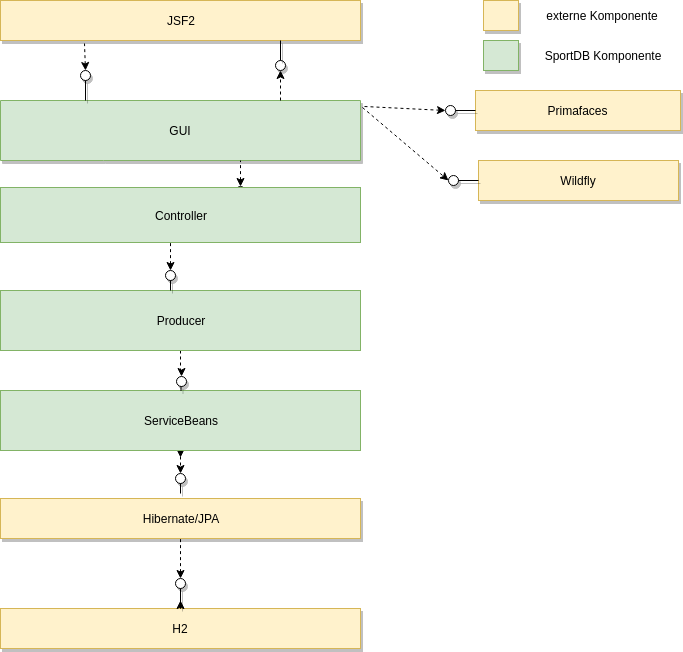
\includegraphics[width=0.9\textwidth]{content/pictures/externdiagram}
	\label{pic:concrete_component_diag}
\end{figure}


